\subsubsection{Singular Spectrum Analysis} \label{link::ssa}
До этого момента все рассмотренные модели использовали в своей основе идею о стационарности, представленную в определении (\myref{def::weak_ts_stationarity}) и (\myref{def::strong_ts_stationarity}). Теперь же рассматриваем иной подход, основанный на отсутствии предпосылок относительно исходных данных. То есть теперь имеющийся набор значений воспринимается как сигнал, характеризующий объект на некотором промежутке времени. Иными словами, нет необходимости предполагать как распределены данные или думать, что все имеющиеся значения - реализации набора случайных величин. Пользуясь определением (\myref{def::signal_stationarity}), рассматриваем следующее преобразование исходного ряда.

Исследуемый метод основывается на сингулярном разложении матрицы траекторий (она же матрица Ханкеля), отборе необходимого количества главных компонент (в методе Principal Component Analysis \cite{abdi2010pca}) и последующей реконструкции (аппроксимации) исходного ряда. Название метода за рубежом - Singular Spectrum Analysis (SSA), в России - Гусеница \cite{catarpillar_ssa}. То есть сам алгоритм SSA имеет 2 этапа: разложение и реконструкция. Рассматриваем каждый их них отдельно.

Пусть дан исходный ряд вида  ${Y = (y_0, ..., y_{N - 1})}$, преобразуем его в матрицу траекторий (Ханкелиан). Для этого выполняем операцию:
\begin{equation} \label{eq::hankelisation}
	Y \rightarrow X \in \R^{L \times K}: L \in [2, \lfloor N / 2 \rfloor], K = N - L + 1
\end{equation}
\noindent Основываясь на методе Singular Vector Decomposition (SVD) \cite{martin2012svd}, получаем декомпозицию:
\begin{equation}
	X = \underbrace{U}_{L \times L} \underbrace{\Sigma}_{L \times K} \underbrace{V^*}_{K \times K}
\end{equation}
Где ${d - \textbf{ранг}(X)}$. Для ортонормальной $V \in \R^{K \times K} \Rightarrow V^{-1} = V^T$ и второй случай: ${V \in \mathbb{C}^{K \times K} \Rightarrow V^* = \left(\overline{V}\right)^T}$ - Эрмитово сопряжение. Столбцы ${U}$ образуют ортонормированный базис в пространстве столбцов X, а столбцы ${V}$ - в пространстве строк X. ${\Sigma}$, в свою очередь, <<диагональная>> матрица, составленная из сингулярных чисел ${XX^T}$ и ${X^TX}$, $T$ - операция транспонирования. Далее замечаем, что разложение  $X$ можно представить в виде суммы элементарных матриц:
\begin{equation} \label{eq::ssa_decomposition}
	X = \sum_{j = 1}^{d} \sigma_j U_j V_j^* = \sum_{j = 1}^{d} \sigma_j \overbrace{U_j}^{L \times 1} \overbrace{V_j^*}^{1 \times K} = \sum_{j = 1}^{d} X_j = \sum_{s \in S} X_s + \sum_{t \in T} X_t + \sum_{o \in O} X_o
\end{equation}
Где $|S| + |T| + |O| = d$, при этом интересно, что $\sigma_j = \sqrt{\lambda_j}$ - где $\lambda_j$ - собственное значение матрицы X, когда она квадратная. Далее, $(\sigma_j, U_j, V_j)$ - вклад $j$-ой собственной тройки в матрицу X. Иначе: как много информации об $X$, где $X$ - Ханкелиан от исходного временного ряда, содержит $j$-я элементарная матрица. $s \in S$ - компоненты сезонности, $t \in T$ - компоненты тренда, $o \in O$ - все остальные компоненты. Важно, что в настоящем исследовании ранее было оговорено, что сезонность в финансовых рядах подобного вида отсутствует, то есть признается наличие только тренда и шума. То есть даже если сезонность присутствует, то ее компоненты относятся к шуму. На данном этапе говорим, что первый пункт плана (декомпозиция) выполнен. Приступаем ко второму - реконструкции.

Очевидно, если сложить все элементарные матрицы, то по (\ref{eq::ssa_decomposition}) получаем исходную матрицу $X$, но это не исходный ряд. Таким образом, встает вопрос \textbf{Q}:  Как из Ханкелиана получить ряд? \textbf{A}: Для этого используется оператор Деханкелизации. 
\begin{equation}
	\begin{split}
		\hat{H}: \; & L\times K \rightarrow N\\
		\tilde{X_j} & = \hat{H}X_j - \text{ элементы на побочной диагонали $\approx$ равны.}\\
		\tilde{X_j} & \stackrel{\text{avg}}{\rightarrow} \tilde{Y_j} - \text{ восстановленный $Y$ через усреднение.}
	\end{split}
\end{equation}
Для получения некоторого ряда из элементарной матрицы применяется также оператор усреднения по побочной диагонали, задаваемый формулой:
\begin{equation} \label{eq::dehankelisation}
	\tilde{x}_{m,n} = 
	\left\{\begin{array}{ll}
		\displaystyle
		\frac{1}{s + 1} \sum_{l = 0}^s x_{l, s - l} & \text{, } 0 \le s \le L - 1\\
		\displaystyle
		\frac{1}{L - 1} \sum_{l = 0}^{L - 1} x_{l, s - l} & \text{, } L \le s \le K - 1\\
		\displaystyle
		\frac{1}{K + L - S - 1} \sum_{l = s - K + 1}^L x_{l, s- l} & \text{, } K \le s \le K + L - 2
	\end{array}\right.
\end{equation}
\noindent Где $s = m + n$. Также интересно, что  $\hat{H}$ является линейным. Доказываем это:
\begin{lemma}
	Оператор деханкелизации $\hat{H}: L \times K \to N$ является линейным.
\end{lemma}
\begin{proof}
	Для того, чтобы оператор являлся линейным необходимо выполнение свойств: 1) $\hat{H}(A + B) = \hat{H}A + \hat{H}B$, где $A, B \in \mathbb{X} \subset \R^{L \times K}$, для которого определен оператор $\hat{H}$ 2) $\hat{H}(\alpha A) = \alpha \hat{H}A$, где $\alpha \in \R$. Рассматриваем по-порядку:
	\begin{enumerate}
		\item Пусть изначально есть 2 ряда $a$ и $b$ длины $N$. После этого они переводятся в матрицу траекторий путем ханкелизации (\ref{eq::hankelisation}). Получаем 2 матрицы $A, B \in \R^{L \times K}$, где на побочной диагонали стоят одинаковые элементы. При этом $L$ не обязательно равно $K$, в таком случае получаем название не <<побочная диагональ>>, а <<антидиагонали>>. После этого $C = A + B$, соответственно на антидиагоналях $C$ стоят одинаковые элементы, таким образом $\hat{H}C = a + b$, но по определению ханкелизации - переходу к матрице траекторий - получаем, что $\hat{H}C = \hat{H}A + \hat{H}B$.
		\item Теперь рассматриваем $\alpha A: \alpha \in R, A \in \R^{L \times K}$. Получаем, что каждый элемент матрицы умножается на $\alpha$, однако, как было сказано в (\ref{eq::dehankelisation}), диагональные элементы усредняются. Таким образом, получаем, что каждый элемент исходного ряда умножается на $\alpha$, но если $\alpha$ везде одинаковое, то просто выносим его из данного вектора, что равносильно $\hat{H}(\alpha A) = \alpha \hat{H}A$.
	\end{enumerate}
\end{proof}

\noindent Из вышедоказанной леммы следует, что:
\begin{equation}
	X = \hat{H}X = \hat{H} \left(\sum_{j = 1}^{d} \sigma_j U_j V_j^*\right) = \sum_{j = 1}^{d} \hat{H}X_j = \sum_{j = 1}^{d} \tilde{X}_j
\end{equation}
\noindent Теперь определяемся с тем, какие именно компоненты (элементарные матрицы) необходимо взять, чтобы получился сигнал, лишенный шума. Теперь главной задачей является избавление от шума, чтобы в итоге восстановленный ряд имел вид:
\begin{equation}
	\hat{Y} = \hat{H} \sum_{t \in T} \sigma_t U_t V^*_t = \sum_{t \in T} \hat{H}X_j 
\end{equation}
\noindent Где $Y - \hat{Y}$, по предположению, шум. \textbf{Q}: Как понять, какие компоненты выбрать? \textbf{A}: корреляционная матрица, построенная на основе взвешенного скалярного произведения. \textbf{Q}: Откуда брать веса? Какими они должны быть? \textbf{A}: В качестве весов используем количество раз, которое каждое число встречается на побочной диагонали элементарной матрицы траекторий. Сам вес задаем формулой:
\begin{equation}
	w_k = \left\{\begin{array}{ll}
		k + 1 & \text{, } 0 \le k \le L - 1\\
		L & \text{, } L \le k \le K - 1\\
		N - k & \text{, } K \le k \le N - 1
	\end{array}\right.
\end{equation}
На основе этих весов строим корреляционную матрицу:
\begin{equation}
	W_{corr} = \left\{ w_{i, j} = \frac{\left(\tilde{Y}_j, \tilde{Y}_i\right)_w}{\lVert \tilde{Y}_i \rVert_w \lVert \tilde{Y}_j \rVert_w} \right\}_{i, j = 0}^{N - 1}: \left(\tilde{Y}_j, \tilde{Y}_i\right)_w = \sum_{k = 0}^{N - 1} w_k \cdot \tilde{y}_{i, k} \cdot \tilde{y}_{j, k}
\end{equation}
$w_{i, j} \rightarrow 1$ если $\tilde{Y}_i$ и $\tilde{Y}_j$ близки, иначе $w_{i, j} \rightarrow 0$. Пороговое значения для группировки задается как гиперпараметр, что делает данный метод менее универсальным, но позволяет решить вопрос выбора компонент. 

Предсказания последующих значений исследуемого ряда происходит по следующему алгоритму \cite{catarpillar_ssa}:
Важно: ${U_j}$ - $j$ столбцы $U$, а ${\tilde{y}_t}$ - реконструированный ряд без компоненты шума.
\begin{enumerate}
	\item Подсчитываем ${r = \lvert \left\{\sigma_j: \sigma_j > 0 \right\} \rvert}$.
	\item Берем ${\left\{ \underline{U}_{j, k} : 1 \le j \le r, 1 \le k < L \right\}: U}$ -  матрица с ортонормированными столбцами.
	\item Берем ${\left\{\pi_j : \pi_j = U_{j, L}: j = \overline{1, r}\right\}}$ - ${\pi_j}$ - последний элемент каждого из $r$ столбца матрицы $U$.
	\item Вычисляем $\nu^2 = \sum_{j = 1}^r \pi_j^2$.
	\item Вычисляем вектор коэффициентов ${R = \left(a_{L - 1}, \ldots, a_{1}\right)^T = \frac{1}{1 - \nu^2} \sum_{j = 1}^r \pi_j \underline{U}_j}: \underline{U}_j \in \R^{L-1 \times 1}$
	\item Для прогнозирования используется формула:
	\begin{equation}
		y_t = 
		\left\{\begin{array}{ll}
			\displaystyle
			\tilde{y}_t & \text{, } t = \overline{1, N}\\
			\displaystyle
			\sum_{j = 1}^{L - 1}a_j y_{t - j} & \text{, } t = \overline{N+1, N + h}
		\end{array}\right.
	\end{equation}
	\noindent Для интереса: более подробно о деталях предсказания временных рядов методом SSA в \cite{catarpillar_ssa}.
\end{enumerate}

Второй этап (реконструкция) тоже закончен, однако остается два вопроса: 1) Чему изначально должна равняться переменная $L$, отвечающая за количество компонент, на которые производится разбиение? 2) Как наиболее точно разделить все компоненты по группам, максимальной удалив шум? Отвечаем на данные вопросы последовательно: 1) Существуют решения и предложения по данному вопросу \cite{catarpillar_ssa}, \cite{wang2015selection}, однако до конца данный вопрос разрешается только, исходя их задачи, к которой применяется SSA 2) Существует еще больше методов, позволяющих произвести подобное разбиение \cite{catarpillar_ssa}, \cite{kuang2020efficient}, \cite{lin2019grouping}, \cite{lin2016grouping}, однако аналогично предыдущему вопросу на этот тоже нет точного ответа. Для примера в настоящем исследовании проводится изучение и реализация алгоритма, описанного в \cite{kuang2020efficient}. Также интересно, что алгоритм предсказания является итерационным, то есть для получения одного нового значения необходимо полностью повторить все действия, что по аналогии сравнимо с <<гусеницей>>.

Главная задача, стоящая перед авторами \cite{kuang2020efficient}, - это предложить устойчивый к входным данным  и эффективный алгоритм <<очищения>> исходного сигнала посредством применения многоразового SSA. Ключевое отличие предложенного метода от непосредственно ручного очищения сигнала - универсальность и отсутствие гиперпараметров. В исходном SSA алгоритме данных параметров целых 2: $L$ - количество компонент и $M$ - количество групп, на которые производится разбиение полученных компонент. Таким образом, встает вопрос о необходимости автоматизации выбора данных параметров или о предложении алгоритма с совершенно иным подходом, лежащим в основе группировки компонент.

Идея метода в итеративном разбиении исходного сигнала посредством классического SSA на $L_1$ компонент и дальнейшей группировке на <<шум>> и не <<шум>>.  То есть сигнал, признанный лишенным шума на шаге  $i$, на шаге $i + 1$ принимается за сигнал с шумом. Таким образом, алгоритм повторяется далее и далее до тех пор, пока не выполняется критерий останова. В случае отсутствия оного, исход алгоритма упирается в количество заданных итераций: возможна ситуация, когда важная компонента, не относящаяся к шуму, из-за большого количество шагов алгоритма классифицируется как шумовая. Следовательно, часть важной информации о сигнале теряется. Если же количество итераций слишком мало, то сигнал все равно остается зашумленным.

На $i$-й итерации сигнал дробится на $L_1$ компонент, а далее оператором $G$ - Grouping разбивается на группы: сигнал и шум. На $i + 1$-й итерации сигнал, признанный лишенным шума на $i$-м этапе опять делится на $L_1$ элементов, после чего все полученные элементы распределяются оператором $G$ на 2 группы. Таким образом, задав $ds_m$ (от denoised signal) - сигнал без шума на итерации $m$, а $o_m$ (от other) - компонента шума на итерации $m$, получаем соотношение:
\begin{equation}
	ds_m = ds_{m + 1} + o_{m + 1}
\end{equation}
Где $m = \overline{1, M}$, $M \in \N$ - общее количество итераций алгоритма. Более того, согласно \cite{kuang2020efficient}, исходный сигнал полноценно восстанавливается в виде:
\begin{equation}
	x = ds_m + n_m = ds_m + \sum_{i = 1}^m o_m
\end{equation}
$n_m$ - накопленные за $m$ шагов компоненты шума. Таким образом, финальный алгоритм по очистке сигнала от шума, представленный в \cite{kuang2020efficient}, имеет вид (aлг.~\ref{alg::signal_denoising_ssa}). 

Алгоритм весьма лаконичен и прост. Ключевая его особенность - критерий останова в строке 6, в которой сказано следующее: <<Вычисляем разницу между сигналами в момент $m$ и $m - 1$, но при этом смотрим, чтобы итоговое значения было больше $0$, что гарантирует сохранение тренда>>. Однако при этом остается один гиперпараметр $M$, задающий общее количество итераций. Он необходим для данного алгоритма, так как без него процесс дробления продолжается бесконечно. Таким образом, наличие цикла for гарантирует конечность алгоритма как такового.
\begin{algorithm}[H]
	\caption{Очистка исходного сигнала от шума} \label{alg::signal_denoising_ssa}
	\begin{algorithmic}[1]
		\Require $x \in R^N$ - исходный сигнал.
		\Require $L_1 = 2$ - размер окна.
		\State Вычисляем: $ds_1$ и $n_1 = o_1$ через $SSA(L_1, G)$
		\State Вычисляем: скалярное произведение $\langle ds_1, n_1 \rangle = \sum_{j = 1}^N ds_{1j} \cdot n_{1j}$
		\For{$m = \overline{1, M}$}
			\State Вычисляем: $ds_m$ и $n_m = \sum_{j = 1}^m o_j$ через $SSA(L_1, G)(ds_{m - 1})$
			\State Вычисляем: скалярное произведение $\langle ds_m, n_m \rangle = \sum_{j = 1}^N ds_{mj} \cdot n_{mj}$
			\If{$\langle ds_m, n_m \rangle - \langle ds_{m - 1}, n_{m - 1} \rangle > 0$}
				\State \textbf{break}
			\EndIf
		\EndFor
		\State \Return оптимальное количество итераций: $m_{opt} = m - 1$, где $m$ - значение, на котором завершился цикл.
		\State \Return сигнал $ds_{m - 1}$, очищенный от шума.
	\end{algorithmic}
\end{algorithm}
\noindent Теперь, основываясь на вышеизложенной теории, рассматриваем практические применение как самого SSA алгоритма, включающего декомпозицию, реконструкцию и предсказание, так и Multistage SSA (MSSA).

\subsubsubsection{Пример: SSA}
\\\\
В качестве искусственных данных исследуем результат применения закона:
\begin{equation} \label{link::illustr_func}
	f(x) = \frac{1}{4}x^2 + \sin(5x) + \cos(x) \cdot \varepsilon: \varepsilon \sim N(0, I_n)
\end{equation}
Где $f: \R^n \to \R^{n}$, а $\varepsilon$ - вектор белого шума, $I_n$ - единичная матрица размера $n \times n$. Графически результат работы данной функции имеет вид:
\begin{figure}[H]
	\centering
	\begin{tikzpicture}
		\begin{axis}[
			grid = both,
			legend pos = north west,
			minor tick num = 1,
			major grid style = {lightgray},
			minor grid style = {lightgray!25},
			%title= {},
			width = \textwidth,
			height = 0.45 \textwidth,
			xmin=-5, xmax=5,
			ymin=-4, ymax=7.5,
			line width=0.3mm
			]
			
			\addplot[opacity = 0.25, color = blue] table [
			x=x, 
			y=y, 
			col sep=comma,
			mark={},
			] {./source/source_csv/Illustration data/ssa/data_to_denoise.csv};
			
			\addplot[domain = -5:5,
			samples = 300,
			color = teal,
			smooth,
			line width = 0.05cm,] {sin(deg(5 * x)) + 1 / 4 * (x^2)};
			
			\legend{$f(x)$, $f(x)$ без шума};
		\end{axis}
	\end{tikzpicture}
	\caption{Построение $f(x)$. см. выражение (\ref{link::illustr_func})}
\end{figure}
В настоящем сигнале присутствуют как трендовая $1/4 \cdot x^2$ и сезонная $\sin(5x)$ составляющие, так и необычный (гетероскедастичный: с различающийся дисперсией) шум $\cos(x) \cdot \varepsilon$. Таким образом, можно уверенно пытаться применить SSA для расщепления данного сигнала на составляющие.

Пусть для начала $L = 20$, то есть количество компонент, на которые проводится расщепление составляет $20$ штук. Для предсказаний используем последние $100$ значений из $2'000$. Тогда общий вид разложения с учетом исходных выглядит следующим образом:
\begin{figure}[H]
	\centering
	\begin{tikzpicture}
		\begin{axis}[
			grid = both,
			legend pos = south east,
			minor tick num = 1,
			major grid style = {lightgray},
			minor grid style = {lightgray!25},
			%title= {},
			width = \textwidth,
			height = 0.45 \textwidth,
			xmin=-5, xmax=5,
			ymin=-4, ymax=7.5,
			line width=0.3mm
			]
			
			\addplot[opacity= 0.25] table [
			x=x, 
			y=y, 
			col sep=comma,
			mark={}
			] {./source/source_csv/Illustration data/ssa/data_to_denoise.csv};
			
			\addplot[domain = -5:5,
			samples = 300,
			color = green,
			smooth,
			line width = 0.05cm] {sin(deg(5 * x)) + 1 / 4 * (x^2)};
			
			\addplot[line width = 0.05cm, color= blue] table [
			x=x, 
			y=y1, 
			col sep=comma,
			mark={},
			] {./source/source_csv/Illustration data/ssa/components.csv};
			
			\addplot table [
			x=x, 
			y=y2, 
			col sep=comma,
			mark={},
			] {./source/source_csv/Illustration data/ssa/components.csv};
			
			\addplot table [
			x=x, 
			y=y3, 
			col sep=comma,
			mark={},
			] {./source/source_csv/Illustration data/ssa/components.csv};
			
			\addplot table [
			x=x, 
			y=y4, 
			col sep=comma,
			mark={},
			] {./source/source_csv/Illustration data/ssa/components.csv};
			
			\addplot table [
			x=x, 
			y=y5, 
			col sep=comma,
			mark={},
			] {./source/source_csv/Illustration data/ssa/components.csv};
			
			\addplot table [
			x=x, 
			y=y6, 
			col sep=comma,
			mark={},
			] {./source/source_csv/Illustration data/ssa/components.csv};
			
			\legend{$f(x)$, $f(x)$ без шума, Компонента 1};
		\end{axis}
	\end{tikzpicture}
	\caption{Декомпозиция $f(x)$. см. выражение (\ref{link::illustr_func})} \label{fig::illustr_decomposition}
\end{figure}
\noindent Большинство компонент показывают себя как гетероскедастичный шум и лишь только одна компонента, соответствующая большему сингулярному числу матрицы Ханкеля от исходного ряда, обозначенная на графике, являет собой нечто похожее на тренд.
\begin{figure}[H]
	\centering
	\begin{tikzpicture}
		\begin{axis}[
			grid = both,
			legend pos = north west,
			minor tick num = 1,
			major grid style = {lightgray},
			minor grid style = {lightgray!25},
			%title= {},
			width = \textwidth,
			height = 0.45 \textwidth,
			xmin=1, xmax=20,
			ymin=0, ymax=0.025,
			line width=0.3mm
			]
			
			\addplot table [
			x=x, 
			y=each, 
			col sep=comma,
			%mark={},
			] {./source/source_csv/Illustration data/ssa/contribution.csv};
			
			\legend{Каждая компонента};
		\end{axis}
	\end{tikzpicture}
	\caption{<<Информативность>> каждой компоненты}
\end{figure}

\begin{figure}[H]
	\centering
	\begin{tikzpicture}
		\begin{axis}[
			grid = both,
			legend pos = north west,
			minor tick num = 1,
			major grid style = {lightgray},
			minor grid style = {lightgray!25},
			%title= {},
			width = \textwidth,
			height = 0.45 \textwidth,
			xmin=1, xmax=20,
			ymin=0.9, ymax=1,
			line width=0.3mm
			]
			
			\addplot[color= red] table [
			x=x, 
			y=cumsum, 
			col sep=comma,
			%mark={},
			] {./source/source_csv/Illustration data/ssa/contribution.csv};
			
			\legend{Накопленная сумма};
		\end{axis}
	\end{tikzpicture}
	\caption{Накопленная <<Информативность>> каждой компоненты}
\end{figure}
Из вкладов каждой из компонент видно, что к сожалению, первая компонента очевидно является тредном и сезонностью, а все остальное - шум, то есть путем дробления на 20 компонент не удалось вычленить тренд и сезонность. Однако интересно, что, исходя из рисунка (\ref{fig::illustr_decomposition}), видно, что почти весь шум, содержащийся в ряде был исключен, что позволяет говорить о выявлении сезонности и тренда почти без шума. Однако слово <<почти>> не дает строгого ответа на вопрос \textbf{Q}:  Сколько именно необходимо компонент, чтобы избавиться от шума? Ведь, возьми мы дробление на большее количество элементов, результат был бы иным. На данный момент останавливаемся на выводе, что 1-я компонента содержит в себе почти всю информацию об исходном графике функции (\myref{link::illustr_func}). 

Далее смотрим на график корреляционной функции между компонентами разложения посредством SSA. Это график (\myref{fig::W_corr_ssa}). Да, действительно, первая компонента является совокупностью треда и сезонности, так как ни с чем не скоррелирована более, чем на $0.3$ (обозначаем это как критерий группировки компонент). Для всех остальных компонент образуется мозаичный график, символизирующий, что настоящая компонента является шумовой и не содержит весомой информации об исходном ряде. Более того, отмечаем, что случайный связи типа $16$ и $2$ со значением $0.48$ являются не более, чем случайными, так как ничего не говорит в пользу обратного при непосредственно визуальном анализе корреляционного графика. По главной диагонали стоят единицы, так как это корреляция самой компоненты с собой. Также отмечаем, что количество <<шума>> увеличивается при визуальном движении к левому-нижнему углу, что не является случайным, так как именно с убыванием величины сингулярного числа (а их именно столько же, сколько компонент - в нашем случае $20$), уменьшается и объем информации, содержащийся в самой компоненте об исходном ряде (сигнале).
\begin{figure}[H]
	\centering
	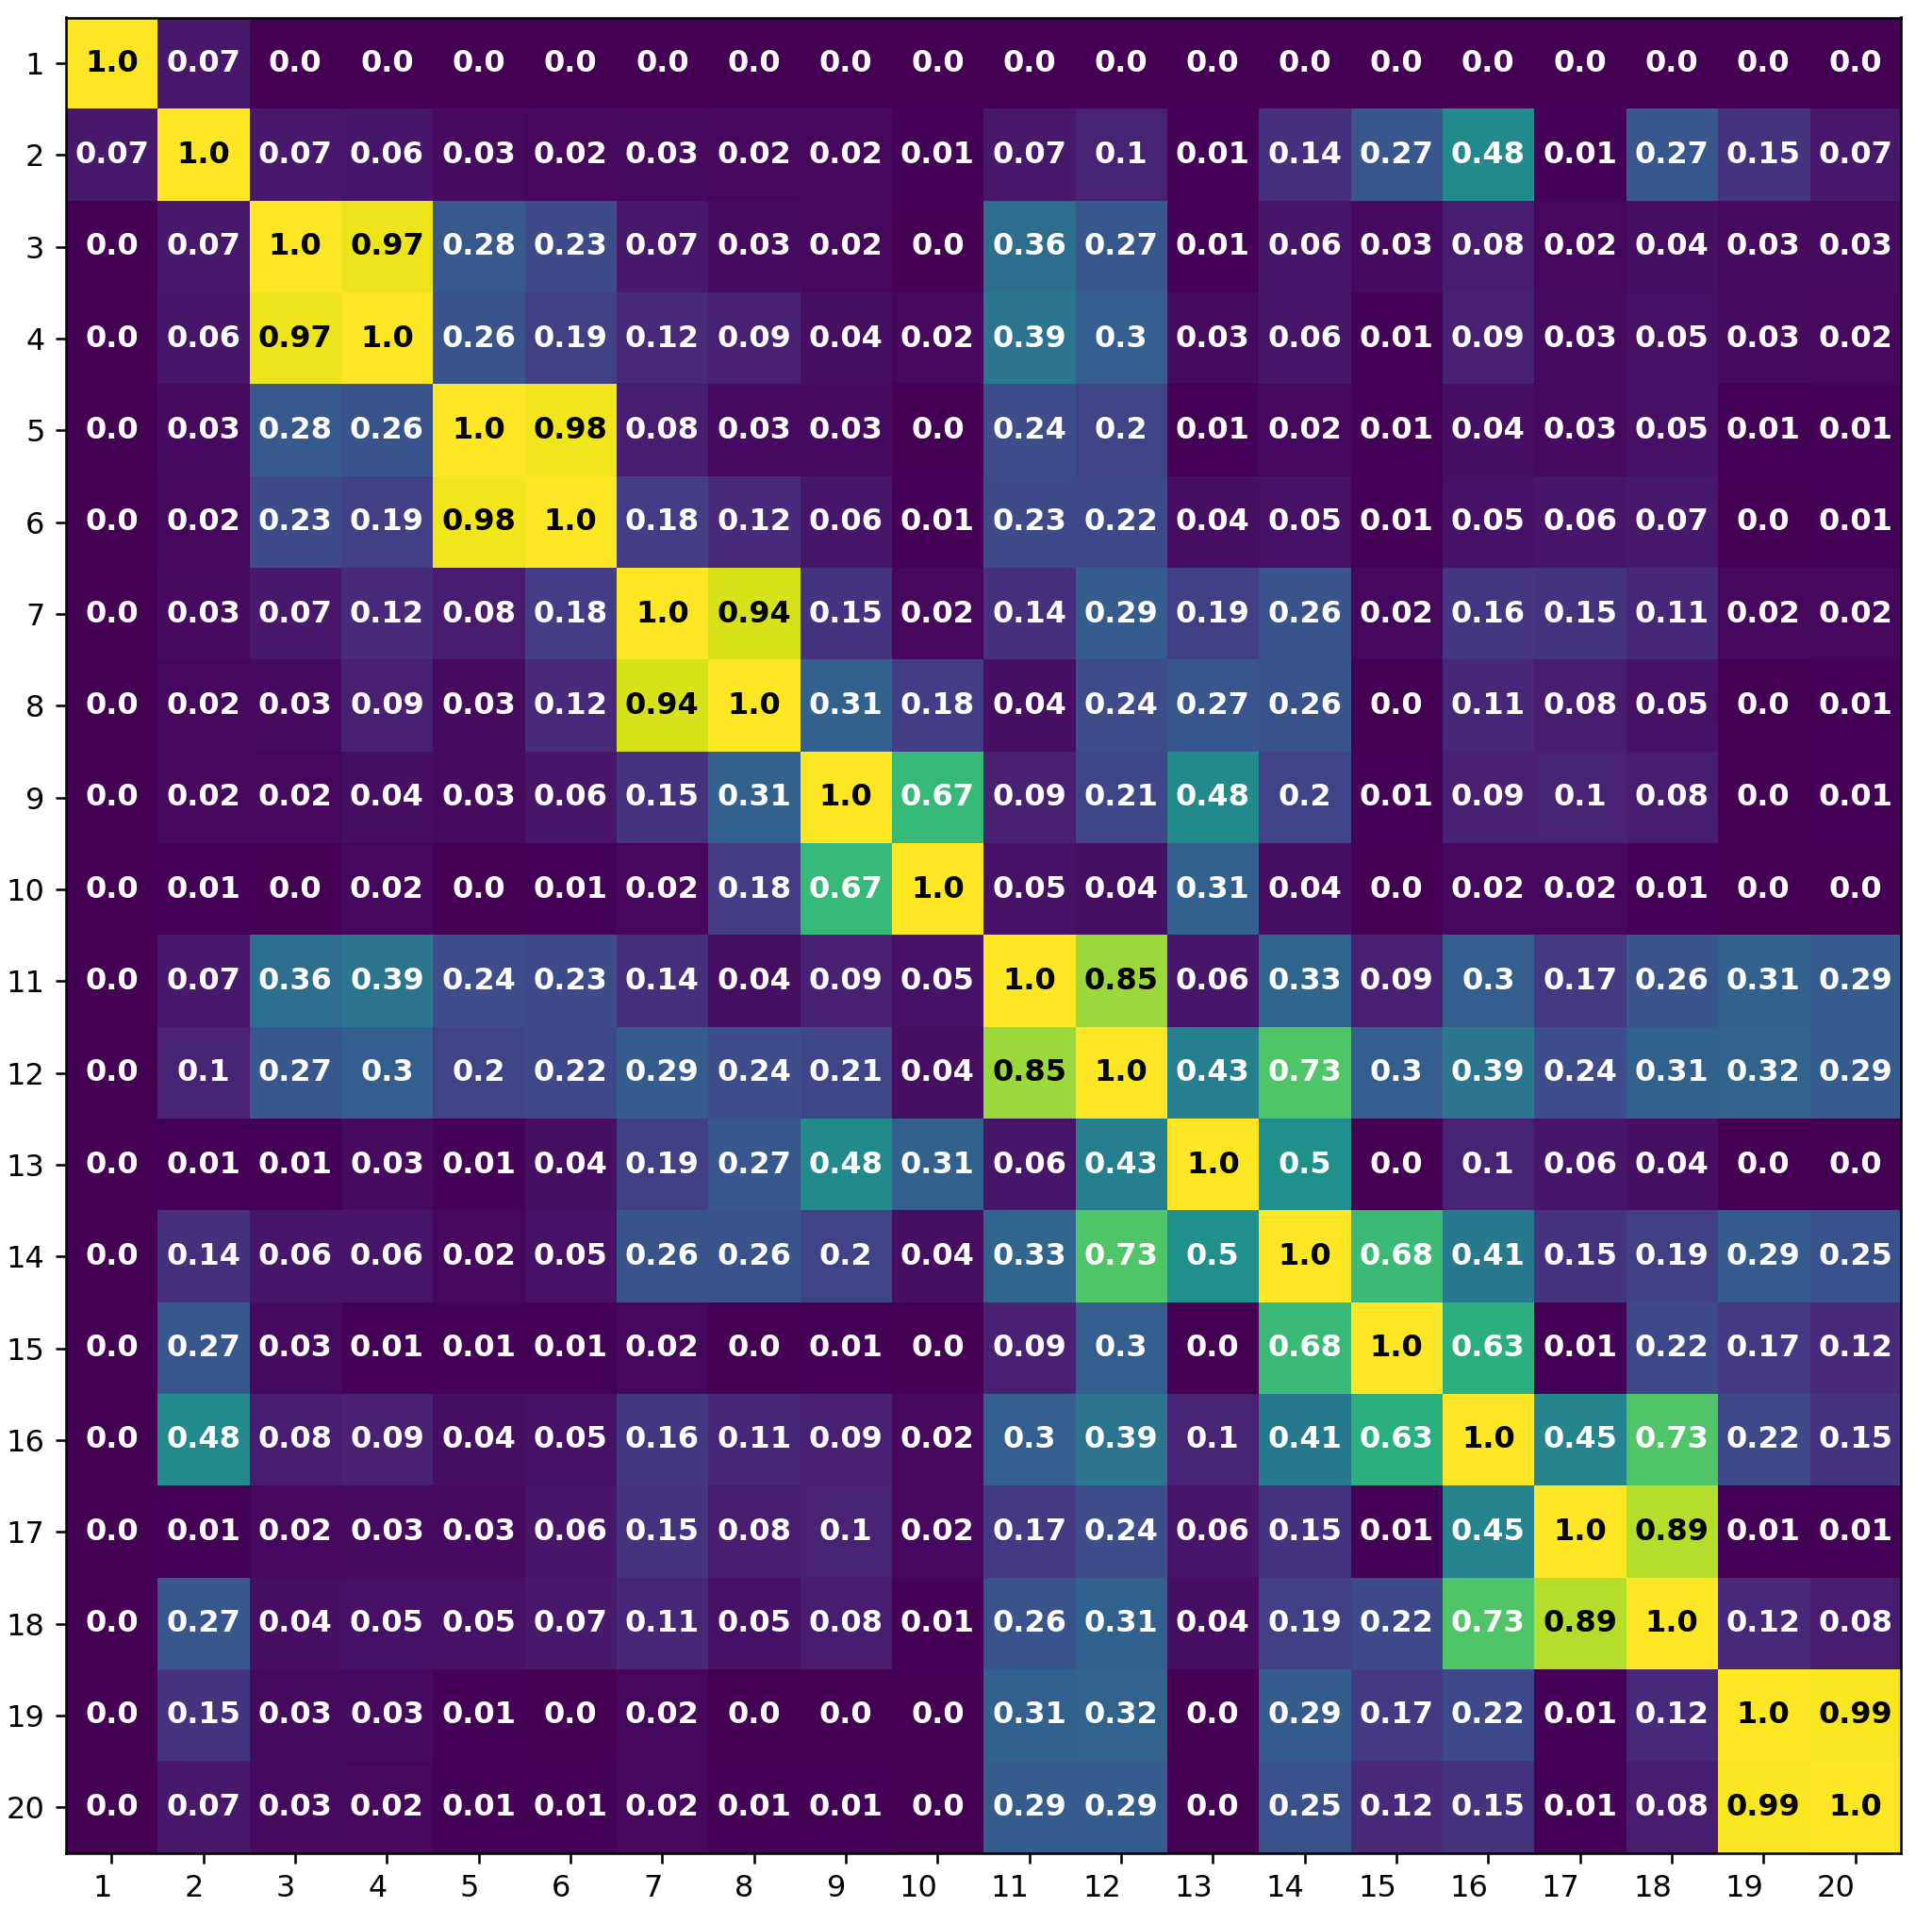
\includegraphics[width=16.5cm, height= 16.5cm]{ssa/W_corr.png}
	\caption{Корреляционная матрица компонент} \label{fig::W_corr_ssa}
\end{figure}

\noindent Финальным пунктом в примере классического SSA является демонстрация его предсказательных способностей.
\begin{figure}[H]
	\centering
	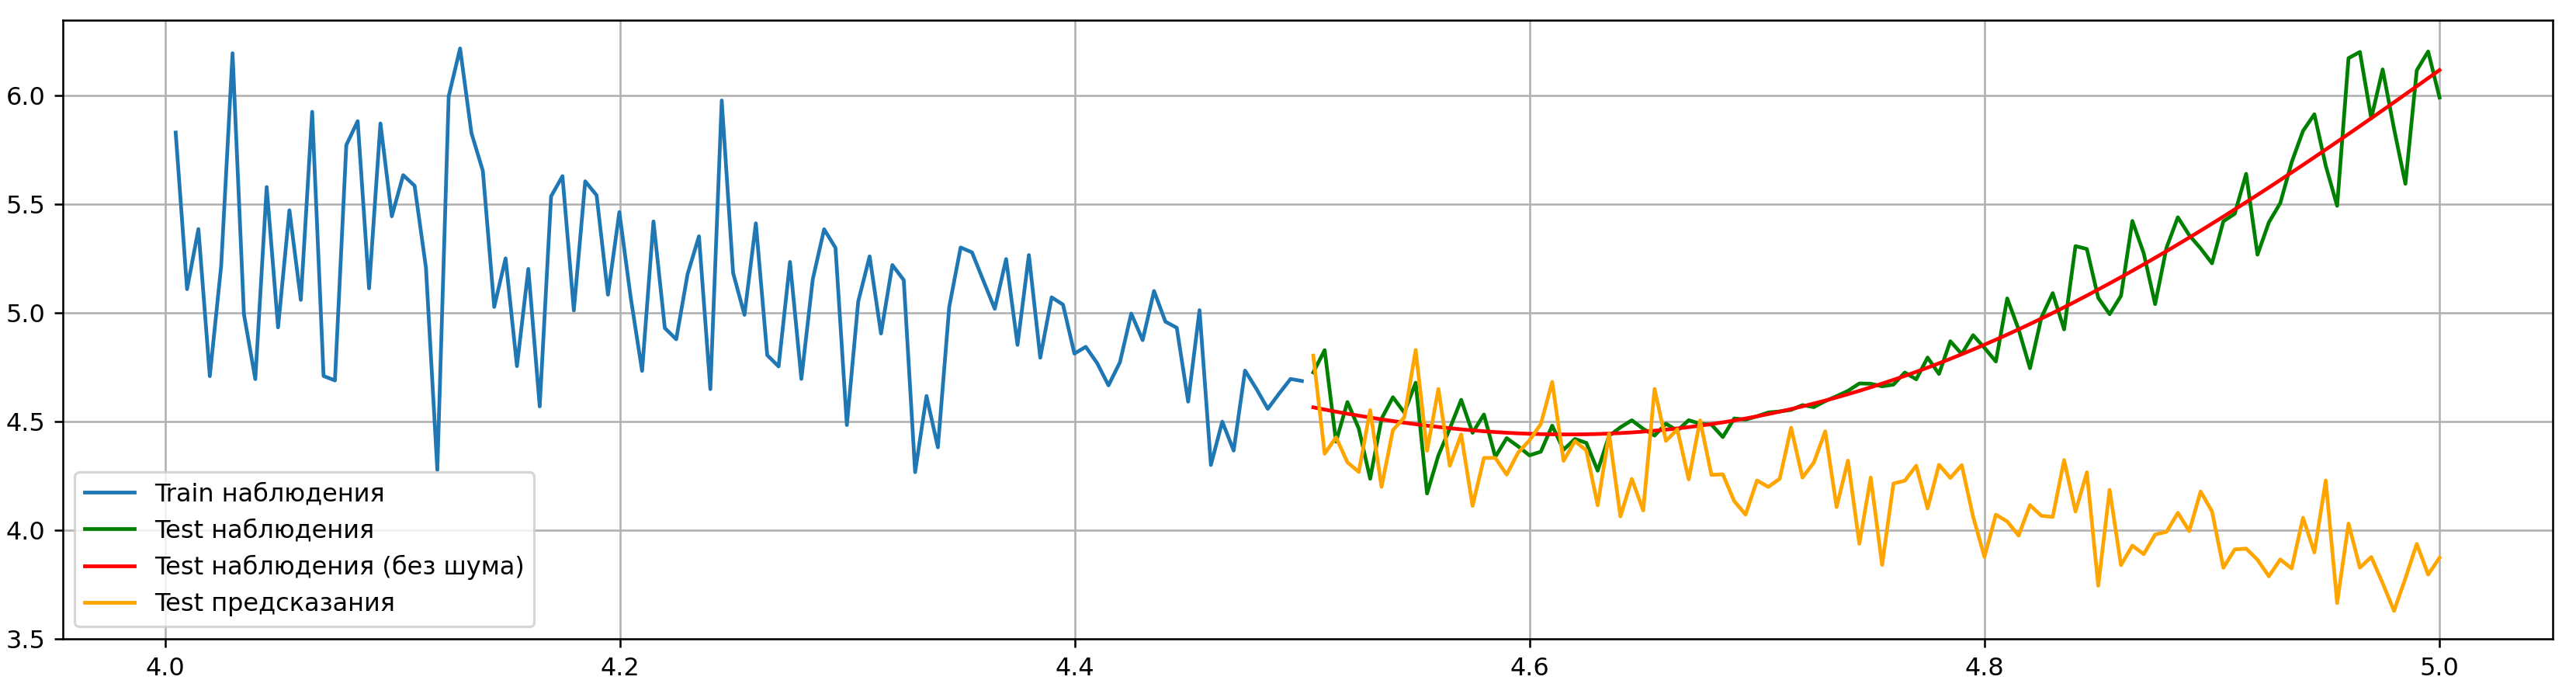
\includegraphics[width=16.5cm]{ssa/forecast_100.png}
	\caption{Прогнозирование значений $f(x)$ на ближайшие $100$ шагов}
\end{figure}
\noindent Анализируя полученные прогнозы, видим, что на начальных этапах они не очень плохи, однако дальше происходит расхождение самого тренда, что в случае с финансовыми рядами, влечет за собой большие риски (под риском понимается потеря денежного эквивалента из-за плохого расчета). Подобная ситуация случилась по 3-м причинам: 1) Малое количество компонент для деления 2) Отсутствие точного алгоритма группировки компонент 3) SSA не использует информацию о самом ряде, что анализирует, а опирается только на техническую составляющую. Однако 1) не говорит, что необходимо дробить ряд на как можно больше компонент, так как данный метод как и любой алгоритм требует как вычислительных мощностей, так и объемов оперативной памяти со стороны персонального компьютера. 2) не утверждает вообще ничего, а 3) упирается к гипотезу о рыночной эффективности и факт, что только техническим анализом невозможно точно предсказать поведение как цены, так и доходности актива соответственно \cite{fama_market_efficiency}. Конечно, 1-3 не утверждают, что SSA не применим вообще, иначе в чем смысл был смысл его создания. Решение - применять SSA конкретно для того, для чего он создавался: для анализа временных рядов - их декомпозиции и аппроксимации. то есть комбинировать его с другими алгоритмами, например, с NN или ARFIMA и так далее везде, где предсказывающая модель чувствительна к шуму в исходных данных. 

\subsubsubsection{Пример: Multistage SSA}
\\\\
Основываясь на алгоритме, предложенном в \cite{kuang2020efficient}, и используя данные, полученные посредством функции (\ref{link::illustr_func}), получаем эффект:
\begin{figure}[H]
	\centering
	\begin{tikzpicture}
		\begin{axis}[
			grid = both,
			legend pos = north west,
			minor tick num = 1,
			major grid style = {lightgray},
			minor grid style = {lightgray!25},
			%title= {},
			width = \textwidth,
			height = 0.45 \textwidth,
			xmin=-5, xmax=5,
			ymin=-4, ymax=7.5,
			line width=0.3mm
			]
			
			\addplot[color = orange, line width = 0.035cm] table [
			x=x, 
			y=denoised, 
			col sep=comma,
			mark={},
			] {./source/source_csv/Illustration data/ssa/denoised.csv};
			
			\addplot[opacity = 0.25, color = blue] table [
			x=x, 
			y=y, 
			col sep=comma,
			mark={},
			] {./source/source_csv/Illustration data/ssa/denoised.csv};
			
			\addplot[domain = -5:5,
			samples = 300,
			color = teal,
			smooth,
			line width = 0.025cm,] {sin(deg(5 * x)) + 1 / 4 * (x^2)};
			
			\legend{$\hat{f}(x)$ - оценка $f(x)$, $f(x)$ c шумом, $f(x)$ без шума};
		\end{axis}
	\end{tikzpicture}
	\caption{Очистка ряда от шума посредством MSSA}
\end{figure}
\noindent Да, очистка от шума не идеальная и существенные отличия от исходного (чистого) ряда, конечно, есть, однако, сравнивая с исходными данными, видим весьма ощутимое различие. Основываясь на этом, делаем вывод, что использование алгоритма MSSA в качестве непараметризованного метода очистки ряда, позволяет назвать сам предложенный метод весьма универсальным. Под <<универсальностью>> понимается отсутствие необходимости вмешательства человека в работу программы. То есть алгоритм делает все сам без помощи из вне. 

Более того, так как одной из основных задач настоящего исследования является написание программы, принимающей на вход некоторый временной ряд, а на выход дающей значение выбранной далее метрики качества для каждой из рассматриваемых моделей, универсальность метода MSSA также как и квази-универсальность (почти универсальность, закрывая глаза на малое количество гиперпараметров) позволяет использовать его в комбинации с другими алгоритмами прогнозирования, в которых конечное значение (прогноз) чувствителен к случайным шокам. Иными словами: очистка от шума необходимо там, где без нее нельзя обойтись для корректного обучения модели на тренировочных данных или там, где от шума возникают серьезные ошибки при построении прогноза. При этом отмечаем, что MSSA применяется только для удаления шума, а не для формирования прогноза как такового.

Таким образом, получаем, что вышеупомянутые алгоритмы очень интересны, функциональны и важны, так как сами по себе не являются зависимыми от некоторой экзогенно заданной модели. Включаем их в финальную таблицу.